\documentclass[a4paper,12pt]{article}
\usepackage[a4paper,top=1.3cm,bottom=2cm,left=1.5cm,right=1.5cm,marginparwidth=0.75cm]{geometry}
\usepackage{cmap}
\usepackage{mathtext}
\usepackage[T2A]{fontenc}
\usepackage[utf8]{inputenc}
\usepackage[english,russian]{babel}
\usepackage{siunitx}

\usepackage{graphicx}

\usepackage{wrapfig}
\usepackage{tabularx}
\usepackage{multirow}

\usepackage{hyperref}
\usepackage[rgb]{xcolor}
\hypersetup{
colorlinks=true,urlcolor=blue
}
\usepackage{amsmath,amsfonts,amssymb,amsthm,mathtools}
\usepackage{icomma}
\mathtoolsset{showonlyrefs=false}
\usepackage{euscript}
\usepackage{mathrsfs}
\DeclareMathOperator{\sgn}{\mathop{sgn}}
\newcommand*{\hm}[1]{#1\nobreak\discretionary{}
{\hbox{$\mathsurround=0pt #1$}}{}}

%%% Заголовок
\author{Макаров Лев Евгеньевич}
\title{Лабораторная работа №2.4.1

Определение теплоты испарения жидкости
}
\date{\today}


\begin{document}

\begin{titlepage}
	\begin{center}
		{\large МОСКОВСКИЙ ФИЗИКО-ТЕХНИЧЕСКИЙ ИНСТИТУТ (НАЦИОНАЛЬНЫЙ ИССЛЕДОВАТЕЛЬСКИЙ УНИВЕРСИТЕТ)}
	\end{center}
	\begin{center}
		{\large Физтех-школа фотоники, электроники и молекулярной физики}
	\end{center}
	
	
	\vspace{4.5cm}
	{\huge
		\begin{center}
			{\bf Отчёт о выполнении лабораторной работы 2.4.1}\\
			Определение теплоты испарения жидкости
		\end{center}
	}
	\vspace{2cm}
	\begin{flushright}
		{\LARGE Автор:\\ Макаров Лев Евгеньевич \\
			\vspace{0.2cm}
			Б04-306}
	\end{flushright}
	\vspace{8cm}
	\begin{center}
		Долгопрудный 2024
	\end{center}
\end{titlepage}

\section{Введение}

\textbf{Цель работы:} 
\begin{enumerate}
	\item измерение давления насыщенного пара жидкости при разной температуре
    \item вычисление по полученным данным теплоты испарения с помощью уравнения Клапейрона–Клаузиуса
\end{enumerate}

\textbf{В работе используются:} 
\begin{itemize}
    \item термостат
    \item герметический сосуд, заполненный исследуемой жидкостью
    \item отсчетный микроскоп
\end{itemize}
\medskip

\section{Теоретические сведения}
  
\begin{wrapfigure}{l}{0.4\textwidth}
    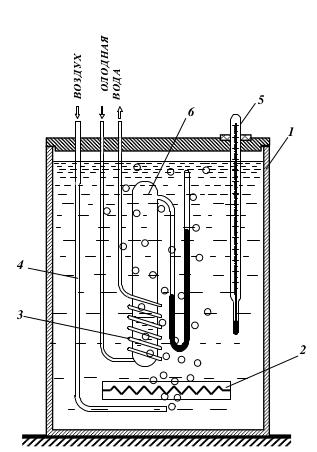
\includegraphics[width=1\linewidth]{ustan.png}
    \centering
    \caption{Схема установки для определения теплоты испарения}
    \label{ust}
\end{wrapfigure}
    
Испарением называется переход вещества из жидкого в газообразное состояние. Оно происходит на свободной поверхности жидкости. При испарении с поверхности вылетают молекулы, образуя над ней пар. Для выхода из жидкости молекулы должны преодолеть силы молекулярного сцепления. Кроме того, при испарении совершается работа против внешнего давления P , поскольку объем жидкости меньше объема пара. Не все молекулы жидкости способны совершить эту работу, а только те из них, которые обладают достаточной кинетической энергией. Поэтому переход части молекул в пар приводит к обеднению жидкости быстрыми молекулами, т. е. к ее охлаждению. Чтобы испарение проходило без изменения температуры, к жидкости нужно подводить тепло. Количество теплоты, необходимое для изотермического испарения одного моля жидкости при внешнем давлении, равном упругости ее насыщенных паров, называется молярной теплотой испарения (парообразования).

Теплоту парообразования жидкостей можно измерить непосредственно при помощи калориметра. Такой метод, однако, не позволяет получить точных результатов из-за неконтролируемых потерь тепла, которые трудно сделать малыми. В настоящей работе для определения теплоты испарения применен косвенный метод, основанный на формуле Клапейрона–Клаузиуса:

\begin{equation}
   \frac{dP}{dT} = \frac{L}{T(V_2-V_1)}.
   \label{1}
\end{equation}

Здесь $P$ -- давление насыщенного пара жидкости при температуре $T$, $T$ -- абсолютная температура жидкости и пара, $L$ -- теплота испарения жидкости, $V_2$ -- объем пара, $V_1$ -- объем жидкости. Найдя из опыта $dP/dT$, $T$, $V_2$ и $V_1$, можно определить $L$ путем расчета. Величины $L$, $V_2$ и $V_1$ в формуле (\ref{1}) должны относиться к одному и тому же количеству вещества; мы будем относить их к одному молю.

В нашем приборе измерения производятся при давлениях ниже атмосферного. В этом случае задача существенно упрощается.

В таблице для ряда жидкостей приведены: температура, при которой давление насыщенных паров равно атмосферному, величины $V_2$ и $V_1$, входящие в (\ref{1}), а также константы $a$ и $b$ в уравнении Вандер-Ваальса.

\begin{figure}[h]
    \centering
    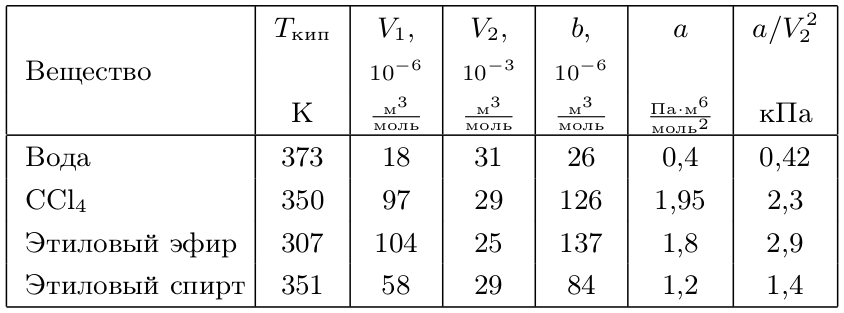
\includegraphics[width=1\textwidth]{table.png}
\end{figure}

Из таблицы видно, что $V_1$ не превосходит 0,5\% от $V_2$. При нашей точности опытов величиной $V_1$ в (\ref{1}) можно пренебречь. Обратимся теперь к $V_2$, которое в дальнейшем будем обозначать просто $V$ . Объем $V$ связан с давлением и температурой уравнением Ван-дер-Ваальса:

\begin{equation}
   \left(P + \frac{a}{V^2}\right)(V - b) = RT.
   \label{2}
\end{equation}

Из рассмотрения таблицы следует, что $b$ одного порядка с $V_1$. В уравнении Ван-дер-Ваальса величиной $b$ следует пренебречь. Пренебрежение членом $a/V^2$ по сравнению с $P$ вносит ошибку менее 3\%. При давлении ниже атмосферного ошибки становятся еще меньше. Таким образом, при давлениях ниже атмосферного уравнение Ван-дер-Ваальса для насыщенного пара мало отличается от уравнения Клапейрона. Положим поэтому

\begin{equation}
   V = \frac{RT}{P}.
   \label{3}
\end{equation}

Подставляя (\ref{3}) в (\ref{1}), пренебрегая $V_1$ и разрешая уравнение относительно $L$, найдем:

\begin{equation}
   L = \frac{RT^2}{P}\frac{dP}{dT} = -R\frac{d(ln P)}{d(1/T)}.
   \label{4}
\end{equation}

В нашем опыте температура жидкости измеряется термометром, давление пара определяется при помощи манометра, а производные $dP/dT$ или $d(ln P )/d(1/T )$ находятся графически как угловой коэффициент касательной к кривой $P(T)$ или соответственно к кривой, у которой по оси абсцисс отложено $1/T$, а по оси ординат $ln P$.


\section{Оборудование и экспериментальные погрешности}

\textbf{Термометр термостата:} $\sigma_t = 0,03$ $C^\circ$ \\
\textbf{Штангенциркуль:} $\sigma_\text{ш} = 0,05$ мм \\

\subsection*{Эксперементальная установка}

Схема установки изображена на рисунке \ref{ust}. Наполненный водой резервуар 1 играет роль термостата. Нагревание термостата производится спиралью 2, подогреваемой электрическим током. Для охлаждения воды в термостате через змеевик 3 пропускается водопроводная вода. Вода в термостате перемешивается воздухом, поступающим через трубку 4. Температура воды измеряется термометром 5. В термостат погружен запаянный прибор 6 с исследуемой жидкостью. Над ней находится насыщенный пар (перед заполнением прибора воздух из него был откачан). Давление насыщенного пара определяется по ртутному манометру, соединенному с исследуемым объемом. Отсчет показаний манометра производится при помощи микроскопа.

\section{Результаты измерений и обработка данных}

\subsection{Предварительные измерения}

с помощью штангенциркуля, к которому прикреплён микроскоп, измерим разность уровней в ртутном U-образном манометре, а также измерим температуру по табло термостата. Результаты измерений запишем в таблицу \ref{data-1}.

\subsection{Измерения при нагревании}

Включим термостат, будем повышать температуру на 1 $C^\circ$ и измерять при этой температуре разность в столбике ртути. Температуру будем повышать до 40 $40^\circ$. Результаты измерений запишем в таблицу \ref{data-1}. Показания температуры переведём в градусы по Кельвину и запишем в таблицу \ref{data-1}.


\begin{table}[!ht]
    \centering
    \begin{tabular}{|l|l|l|l|l|l|l|}
    \hline
        $№$ & $t$, $C^\circ$ & $T$, K & $h_1$, мм & $h_2$, мм & $\Delta h$, мм & $P$, Па \\ \hline
        1 & 23,00 & 296,16 & 74,50 & 93,60 & 19,10 & 2548 \\ \hline
        2 & 24,00 & 297,16 & 74,45 & 93,70 & 19,25 & 2568 \\ \hline
        3 & 25,00 & 298,16 & 74,20 & 94,10 & 19,90 & 2655 \\ \hline
        4 & 26,00 & 299,16 & 73,20 & 95,05 & 21,85 & 2915 \\ \hline
        5 & 27,00 & 300,16 & 72,35 & 95,90 & 23,55 & 3142 \\ \hline
        6 & 28,00 & 301,16 & 71,70 & 96,70 & 25,00 & 3335 \\ \hline
        7 & 29,00 & 302,16 & 70,80 & 97,80 & 27,00 & 3602 \\ \hline
        8 & 30,00 & 303,16 & 70,15 & 98,65 & 28,50 & 3802 \\ \hline
        9 & 31,00 & 304,16 & 69,30 & 99,60 & 30,30 & 4043 \\ \hline
        10 & 32,00 & 305,16 & 68,40 & 100,35 & 31,95 & 4263 \\ \hline
        11 & 33,00 & 306,16 & 67,85 & 101,45 & 33,60 & 4483 \\ \hline
        12 & 34,00 & 307,16 & 66,65 & 102,55 & 35,90 & 4790 \\ \hline
        13 & 35,00 & 308,16 & 65,60 & 103,40 & 37,80 & 5043 \\ \hline
        14 & 36,00 & 309,16 & 64,85 & 104,60 & 39,75 & 5303 \\ \hline
        15 & 37,00 & 310,16 & 63,90 & 105,90 & 42,00 & 5604 \\ \hline
        16 & 38,00 & 311,16 & 62,50 & 107,05 & 44,55 & 5944 \\ \hline
        17 & 39,00 & 312,16 & 61,00 & 108,80 & 47,80 & 6377 \\ \hline
        18 & 40,00 & 313,16 & 60,15 & 109,70 & 49,55 & 6611 \\ \hline
    \end{tabular}\caption{\textit{Измерение давления пара от теммпературы при нагревании}}\label{data-1}
\end{table}


Погрешность измерения разности в столбике ртути равна $\sigma_{\Delta h} = \sqrt{2}\sigma_\text{ш} \approx 0,07$ мм.

Давление водяного пара $P$ можно посчитать по формуле:

\begin{equation}
    P = \rho g \Delta h
\end{equation}

где $\rho$ -- плотность ртути, $g$ -- ускорение свободного падения, а $\Delta h$ -- разность в ртутном столбике. Давление для каждого измерения посчитаем и запишем в таблицу \ref{data-1}.

Погрешность измерения давления давления можно вычислить по формуле:

\begin{equation}
    \sigma_P = \rho g \sigma_{\Delta h} \approx 9 \ \text{Па}
\end{equation}

\subsection{Измерения при охлаждении}

Теперь, охлаждая термостат, будем делать аналогичные измерения. Замерять будем с шагом 2 $C^\circ$. Все измерения запишем в таблицу \ref{data-2}.

\begin{table}[!ht]
    \centering
    \begin{tabular}{|l|l|l|l|l|l|l|}
    \hline
        $№$ & $t$, $C^\circ$ & $T$, K & $h_1$, мм & $h_2$, мм & $\Delta h$, мм & $P$, Па \\ \hline
        1 & 39,00 & 312,16 & 60,50 & 109,40 & 48,90 & 6524 \\ \hline
        2 & 37,00 & 310,16 & 62,55 & 106,90 & 44,35 & 5917 \\ \hline
        3 & 35,00 & 308,16 & 64,80 & 104,50 & 39,70 & 5297 \\ \hline
        4 & 33,00 & 306,16 & 66,95 & 102,10 & 35,15 & 4690 \\ \hline
        5 & 31,00 & 304,16 & 68,55 & 99,90 & 31,35 & 4183 \\ \hline
        6 & 29,00 & 302,16 & 70,20 & 97,20 & 27,00 & 3602 \\ \hline
        7 & 27,00 & 300,16 & 71,70 & 96,45 & 24,75 & 3302 \\ \hline
        8 & 25,00 & 298,16 & 72,95 & 94,85 & 21,90 & 2922 \\ \hline
    \end{tabular}\caption{\textit{Измерение давления пара от теммпературы при охлаждении}}\label{data-2}
\end{table}


\subsection{Обработка данных}

Из формулы \eqref{4} видно, что зависимость $1/T$ от $\ln{P}$ -- линейная. То есть для построения графика зависимости $1/T$ от $\ln{P}$ можно воспользоваться МНК, где $y = \ln{P}$, а $x = 1/T$. Для аппроксимации наилучшей прямой воспользуемся формулой:

\begin{equation}\label{mnk}
    k = \frac{\langle xy\rangle - \langle x \rangle \langle y \rangle}{\langle x^2 \rangle - \langle x \rangle^2},
    \ \text{а} \ \  b = \langle y \rangle - k\langle x \rangle
\end{equation}

Погрешности для $k$ и $b$ рассчитываются по формулам:

\begin{equation}
    \sigma_k = \frac{1}{\sqrt{n}} \sqrt{\frac{\langle y^2 \rangle - \langle y \rangle^2}{\langle x^2 \rangle - \langle x \rangle^2} - k^2}
\end{equation}

\begin{equation}
    \sigma_b = \sigma_k\sqrt{\langle x^2 \rangle - \langle x \rangle^2}
\end{equation}

Посчитаем все необходимые значения для МНК и запишем их в таблицы \ref{mnk-1} и \ref{mnk-2} для нагревания и охлаждения соответственно (перед этим посчитаем значения $1/T$ и $\ln{P}$ и запишем в те же таблицы).


\begin{table}[!h]
    \centering
    \begin{tabular}{|l|l|l|l|l|l|}
    \hline
        N & $1/T$ & $\ln{P} $& $(1/T)^2$ & $\ln^2{P}$ & $\ln{P} \cdot 1/T$ \\ \hline
        1 & 0,0033766 & 7,84316 & 0,00001140 & 61,5152 & 0,02648 \\ \hline
        2 & 0,0033652 & 7,85098 & 0,00001132 & 61,6379 & 0,02642 \\ \hline
        3 & 0,0033539 & 7,88419 & 0,00001125 & 62,1605 & 0,02644 \\ \hline
        4 & 0,0033427 & 7,97767 & 0,00001117 & 63,6433 & 0,02667 \\ \hline
        5 & 0,0033316 & 8,05260 & 0,00001110 & 64,8443 & 0,02683 \\ \hline
        6 & 0,0033205 & 8,11235 & 0,00001103 & 65,8102 & 0,02694 \\ \hline
        7 & 0,0033095 & 8,18931 & 0,00001095 & 67,0648 & 0,02710 \\ \hline
        8 & 0,0032986 & 8,24338 & 0,00001088 & 67,9533 & 0,02719 \\ \hline
        9 & 0,0032877 & 8,30462 & 0,00001081 & 68,9667 & 0,02730 \\ \hline
        10 & 0,0032770 & 8,35764 & 0,00001074 & 69,8502 & 0,02739 \\ \hline
        11 & 0,0032663 & 8,40800 & 0,00001067 & 70,6944 & 0,02746 \\ \hline
        12 & 0,0032556 & 8,47421 & 0,00001060 & 71,8122 & 0,02759 \\ \hline
        13 & 0,0032451 & 8,52578 & 0,00001053 & 72,6889 & 0,02767 \\ \hline
        14 & 0,0032346 & 8,57608 & 0,00001046 & 73,5492 & 0,02774 \\ \hline
        15 & 0,0032241 & 8,63114 & 0,00001040 & 74,4966 & 0,02783 \\ \hline
        16 & 0,0032138 & 8,69008 & 0,00001033 & 75,5176 & 0,02793 \\ \hline
        17 & 0,0032035 & 8,76050 & 0,00001026 & 76,7463 & 0,02806 \\ \hline
        18 & 0,0031933 & 8,79645 & 0,00001020 & 77,3776 & 0,02809 \\ \hline
        ср & 0,0032833 & 8,31545 & 0,00001078 & 69,2405 & 0,02729 \\ \hline
    \end{tabular}\caption{\textit{Вычисление промежуточных значений для МНК при нагревании}}\label{mnk-1}
\end{table}

\begin{table}[!h]
    \centering
    \begin{tabular}{|l|l|l|l|l|l|}
    \hline
        N & $1/T$ & $\ln{P} $& $(1/T)^2$ & $\ln^2{P}$ & $\ln{P} \cdot 1/T$ \\ \hline
        1 & 0,0032035 & 8,78325 & 0,00001026 & 77,1455 & 0,02814 \\ \hline
        2 & 0,0032241 & 8,68558 & 0,00001040 & 75,4394 & 0,02800 \\ \hline
        3 & 0,0032451 & 8,57482 & 0,00001053 & 73,5276 & 0,02783 \\ \hline
        4 & 0,0032663 & 8,45310 & 0,00001067 & 71,4548 & 0,02761 \\ \hline
        5 & 0,0032877 & 8,33869 & 0,00001081 & 69,5337 & 0,02742 \\ \hline
        6 & 0,0033095 & 8,18931 & 0,00001095 & 67,0648 & 0,02710 \\ \hline
        7 & 0,0033316 & 8,10230 & 0,00001110 & 65,6472 & 0,02699 \\ \hline
        8 & 0,0033539 & 7,97996 & 0,00001125 & 63,6797 & 0,02676 \\ \hline
        ср & 0,0032777 & 8,38838 & 0,00001075 & 70,4366 & 0,02748 \\ \hline
    \end{tabular}\caption{\textit{Вычисление промежуточных значений для МНК при охлаждении}}\label{mnk-2}
\end{table}

Теперь можно вычислить коэффициенты наклона прямых и их погрешности для обеих серий измерений согласно формуле \eqref{mnk}.

После подсчёта коэффициентов построим обе наилучшие прямые на одном графике и нанесём туда экспериментальные точкию.

\begin{equation}
    k_\text{н} = \frac{0,02729 - 0,0032833 \cdot 8,31545}{0,00001078 - {0,0032833}^2} \approx -5466 \ \text{К}
\end{equation}

\begin{equation}
    b_\text{н} = 8,31545 - (-5466) \cdot 0,0032833 \approx 26,263
\end{equation}

\begin{equation}
    \sigma_{k_\text{н}} = \frac{1}{\sqrt{18}} \sqrt{
    \frac{69,2405 - {8,31545}^2}{0,00001078 - {0,0032833}^2} - (-5466)^2
    } \approx 70 \ \text{К}
\end{equation}

\begin{equation}
    \sigma_{b_\text{н}} = 70 \sqrt{0,00001078 - {0,0032833}^2} \approx 0,004
\end{equation}

\begin{equation}
    k_\text{о} = \frac{0,02748 - 0,0032777 \cdot 8,38838}{0,00001075 - {0,0032777}^2} \approx -5436 \ \text{К}
\end{equation}

\begin{equation}
    b_\text{о} = 8,38838 - (-5436) \cdot 0,0032777 \approx 26,205
\end{equation}

\begin{equation}
    \sigma_{k_\text{о}} = \frac{1}{\sqrt{8}} \sqrt{
    \frac{70,4366 - {8,38838}^2}{0,00001075 - {0,0032777}^2} - (-5436)^2
    } \approx 80 \ \text{К}
\end{equation}

\begin{equation}
    \sigma_{b_\text{о}} = 80 \sqrt{0,00001075 - {0,0032777}^2} \approx 0,004
\end{equation}

Воспользуемся формулой \eqref{4} найдём $L$ из обоих наборов измерений:

\begin{equation}
    L = - R \frac{d(\ln{P})}{d(1/T)} = -R \frac{d}{d(1/T)} \left( k \cdot (1/T) + b \right) = -R k
\end{equation}

Тогда погрешность вычисления $L$

\begin{equation}
    \sigma_L = R \sigma_k
\end{equation}

\begin{equation}
    L_1 = -R k_\text{н} = -8,31 \cdot (-5466) = 45426 \ \frac{\text{Дж}}{\text{моль}} \ \ \ \sigma_{L_1} = R \sigma_{k_\text{н}} = 8,31 \cdot 70 = 581 \ \frac{\text{Дж}}{\text{моль}}
\end{equation}

\begin{equation}
    L_2 = -R k_\text{н} = -8,31 \cdot (-5436) = 45171 \ \frac{\text{Дж}}{\text{моль}} \ \ \ \sigma_{L_2} = R \sigma_{k_\text{н}} = 8,31 \cdot 80 = 663 \ \frac{\text{Дж}}{\text{моль}}
\end{equation}

Отсюда $L_1 = (45,4 \pm 0,6) \ \text{кДж}/\text{моль}$ и $L_2 = (45,1 \pm 0,7) \ \text{кДж}/\text{моль}$. Как видно значения совпадают в пределах погрешности, но значение, полученное из первой серии измерений, получилось точнее благодаря большему количеству измерений. Тогда значение теплоты испарения возьмём как среднее:

\begin{equation}
    L = (45300 \pm 600) \ \frac{\text{Дж}}{\text{моль}}
\end{equation}

\section{Обсуждение результатов и выводы}

В ходе работы было измерено давление насыщенного пара воды при разной температуре, сначала при увеличении температуры, а потом при уменьшении. По этим данным было вычислено значение теплоты испарения воды для обоих наборов измерений, значения совпали в пределах погрешности.

Табличное значение теплоты парообразования $L_\text{табл} = 40600 \ \text{Дж}/\text{моль}$. Экспериментальные значения сильно превышают табличное. Это скорее всего связпно с тем, что температура жидкости не успевала устояться в ходе измерений, поэтому при записи показаний измеренной давление не соответствует температуре жидкости при этом.

С данной установкой и при данных условиях проведения провести точные измерения невозможно.


\newpage

\begin{figure}[h!]
        \centering
	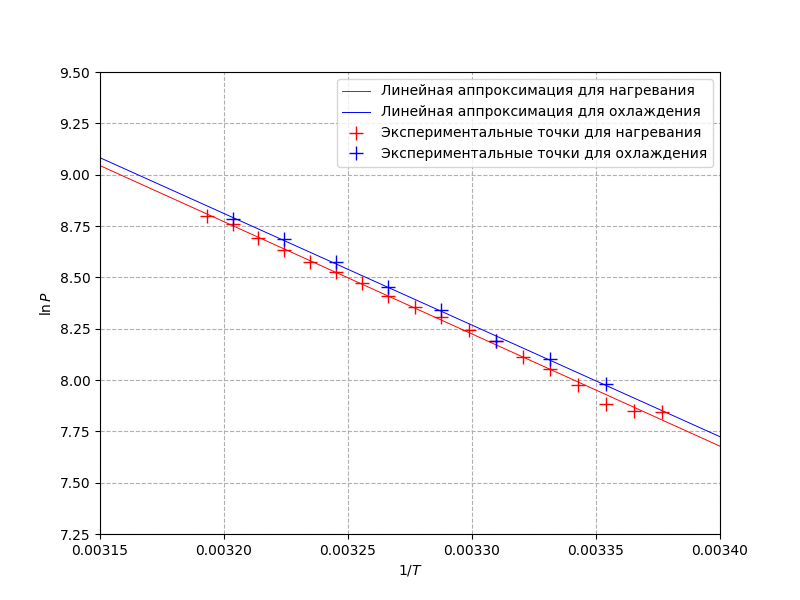
\includegraphics[width=1.1\textwidth]{graph.png}
	\caption{\textit{График зависимости $\ln{P}$ от $1/T$ для обоих наборов измерений}}
	\label{graph}
\end{figure}



\end{document}